\documentclass{standalone}
\usepackage{tikz}
\usetikzlibrary{automata,positioning}
\tikzset{
    state/.style={
        circle,
        draw,
        minimum size=20pt,
        inner sep=0pt
    },
    accepting/.style={
        double,
        double distance=2pt
    },
    initial/.style={
        initial by arrow,
        initial distance=7pt,
        initial text={}
    }
}

\begin{document}
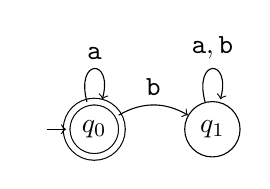
\begin{tikzpicture}[baseline=(current bounding box.center)]
\node[state,initial,accepting] (q0) at (0,0) {$q_0$};
\node[state] (q1) at (1.5,0) {$q_1$};
\path[->] 
  (q0) edge[loop above] node {$\mathtt{a}$} ()
  (q0) edge[bend left] node[above] {$\mathtt{b}$} (q1);
\path[->]
  (q1) edge[loop above] node {$\mathtt{a,b}$} ();
\end{tikzpicture}
\end{document}